\documentclass[11pt]{article}
\usepackage[a4paper,margin=1in]{geometry}
\usepackage{amsmath,amssymb,amsthm}
\usepackage{tikz}
\usepackage{xcolor}
\usepackage[hidelinks]{hyperref}
\hypersetup{pdftitle={When a product state stays a product state},pdfauthor={Vamshi Jandhyala}}
\setlength{\parskip}{0.4em}
\setlength{\parindent}{0pt}

\newtheorem{theorem}{Theorem}
\newtheorem{lemma}[theorem]{Lemma}
\newtheorem{proposition}[theorem]{Proposition}
\newtheorem{corollary}[theorem]{Corollary}
\theoremstyle{remark}
\newtheorem*{remark}{Remark}
\newtheorem*{example}{Example}

\definecolor{inkblue}{RGB}{40,76,105}
\definecolor{softblue}{RGB}{226,235,243}
\definecolor{rust}{RGB}{153,70,45}

\newcommand{\C}{\mathbb{C}}
\newcommand{\R}{\mathbb{R}}
\newcommand{\Z}{\mathbb{Z}}
\newcommand{\N}{\mathbb{N}}
\newcommand{\ip}[2]{\langle #1,#2\rangle}

\title{When a product state stays a product state}
\author{Vamshi Jandhyala}
\date{Preprint v1, 20 October 2026}

\begin{document}
\maketitle
\vspace{-2em}

\begin{abstract}
Let $H$ be a Hamiltonian on $\C^m\otimes\C^n$ and let $a\otimes b$ be a product state whose
evolution $e^{-itH}(a\otimes b)$ is a product state at every time $t$. We show that the same
trajectory is generated by a time-independent local Hamiltonian: there are Hermitian $h_A$
and $h_B$ with $e^{-itH}(a\otimes b)=e^{-ith_A}a\otimes e^{-ith_B}b$ for all real $t$. No
assumption is made on the spectrum of $H$; degenerate eigenvalues and resonant frequencies
are allowed. By induction the same holds for any number of parties. Local generators that
depend on time were known to exist; the content here is that a constant one always does.
The hypothesis cannot be weakened to constant entanglement: an isotropic exchange coupling in a
field keeps the Schmidt coefficients of a suitable two-qubit state fixed for all time, yet no
constant local Hamiltonian generates its trajectory; for two qubits that stay maximally
entangled, a constant local generator does exist. The proof of the main theorem turns the
trajectory into a matrix of polynomials on a torus, factors it in a
unique factorisation domain, and reads off orthogonality from a grading argument. The
algebraic core and the passage from exponential sums to polynomials are formally verified
in Lean.
\end{abstract}

\section{The question}

Two qubits interact through $H=Z\otimes Z$, where $Z=\mathrm{diag}(1,-1)$. Start them in
$\lvert 0\rangle\otimes\lvert +\rangle$, with $\lvert\pm\rangle=(\lvert 0\rangle\pm\lvert
1\rangle)/\sqrt2$. Since $Z\lvert 0\rangle=\lvert 0\rangle$,
\[
e^{-itZ\otimes Z}\bigl(\lvert 0\rangle\otimes\lvert +\rangle\bigr)
=\lvert 0\rangle\otimes e^{-itZ}\lvert +\rangle ,
\]
so the state never becomes entangled, even though $H$ has no local part at all. The motion is
exactly what the local Hamiltonian $h_A=0$, $h_B=Z$ would produce.

A second example has more symmetry. Let $H=J(X\otimes X+Y\otimes Y+Z\otimes Z)+B(Z\otimes
1+1\otimes Z)$, the isotropic exchange coupling in a uniform field. The exchange term equals
$1$ on the symmetric subspace, so for every single-qubit state $\phi$,
\[
e^{-itH}(\phi\otimes\phi)=e^{-it(BZ+J)}\phi\otimes e^{-itBZ}\phi ,
\]
again a product at all times, generated by $h_A=BZ+J$ and $h_B=BZ$.

In both examples the interaction is invisible to one particular state, and the trajectory is
the trajectory of a local, time-independent Hamiltonian. The question, asked on Physics Stack
Exchange~\cite{SE816017}, is whether this is always so.

\begin{theorem}\label{thm:main}
Let $H$ be a Hermitian operator on $\C^m\otimes\C^n$ and let $a\in\C^m$, $b\in\C^n$ be
nonzero. If $e^{-itH}(a\otimes b)$ is a product vector for every $t\in\R$, then there are
Hermitian operators $h_A$ on $\C^m$ and $h_B$ on $\C^n$ such that
\[
e^{-itH}(a\otimes b)=e^{-ith_A}a\otimes e^{-ith_B}b\qquad\text{for all }t\in\R .
\]
\end{theorem}

The hypothesis is about one trajectory only; $H$ may entangle every other product state.
Nothing is assumed about the spectrum of $H$. This matters, because the most direct argument
breaks down at resonances. If $H$ has eigenvalues $0,1,2$ then the frequency $2$ arises both
as $0+2$ and as $1+1$, and a cancellation between the two could in principle hold a state on
the set of product vectors without any local mechanism. The proof below never compares sums of
frequencies, and resonances play no role.

Without the words ``time-independent'' the statement is easy and known. Durt~\cite{Durt2001}
shows that a product state stays a product state exactly when $H$ never couples it to a product
state biorthogonal to it, and that it then follows the local but time-dependent mean-field
Hamiltonians $H_A^{\mathrm{eff}}(t)$ and $H_B^{\mathrm{eff}}(t)$ obtained by partial traces
against the current state of the other party; see also~\cite{Durt2004}. Sperling and
Walmsley~\cite{SperlingWalmsley} derive the same kind of equations of motion for separable
trajectories. In these constructions the generator of each factor depends on the state of the
other factor and therefore on $t$. Theorem~\ref{thm:main} says that a constant generator
always exists. The case where every product state stays a product state is classical: then
$H$ itself is a sum of local terms~\cite{Durt2001}.

Two consequences are immediate. The first answers the question as it was asked, for any number
of parties; the reduction to two parties was pointed out in the comments of~\cite{SE816017} by
Norbert Schuch.

\begin{corollary}\label{cor:multi}
Let $H$ be Hermitian on $\C^{d_1}\otimes\cdots\otimes\C^{d_N}$ and let $\psi_0=a_1\otimes\cdots
\otimes a_N$. If $e^{-itH}\psi_0$ is a product vector across all $N$ factors for every $t$,
then there are Hermitian $h_1,\dots,h_N$, each acting on one factor, with $e^{-itH}\psi_0=
e^{-ith_1}a_1\otimes\cdots\otimes e^{-ith_N}a_N$ for all $t$.
\end{corollary}

\begin{proof}
Induction on $N$. Apply Theorem~\ref{thm:main} to the cut between the first factor and the
rest: $e^{-itH}\psi_0=e^{-ith_1}a_1\otimes e^{-itH'}(a_2\otimes\cdots\otimes a_N)$ with $H'$
Hermitian on the last $N-1$ factors. A product vector determines its factors up to scalars,
so $e^{-itH'}(a_2\otimes\cdots\otimes a_N)$ is a product across the last $N-1$ factors for
every $t$, and the induction hypothesis applies to $H'$.
\end{proof}

\begin{corollary}\label{cor:cyclic}
In the setting of Theorem~\ref{thm:main}, let $K$ be the smallest $H$-invariant subspace
containing $a\otimes b$. Then $H$ and $G=h_A\otimes 1+1\otimes h_B$ agree on $K$.
\end{corollary}

\begin{proof}
The trajectories $e^{-itH}(a\otimes b)$ and $e^{-itG}(a\otimes b)$ coincide, so all their
derivatives at $t=0$ coincide: $H^r(a\otimes b)=G^r(a\otimes b)$ for every $r\ge0$. These
vectors span $K$, and $H$ maps each of them to $H^{r+1}(a\otimes b)=G^{r+1}(a\otimes b)$,
which is where $G$ maps it too.
\end{proof}

So the two examples above are typical: a product trajectory always lives in a subspace on
which the Hamiltonian is secretly local.

\paragraph{The route.} A product state is a rank-one matrix, so the hypothesis says that a
matrix-valued exponential sum has rank one at every time. If all the frequencies were integers,
this sum would be a matrix of polynomials in $z=e^{-it}$ evaluated on the unit circle, rank one
on the circle and therefore rank one as a polynomial matrix. In general we choose a basis of the
frequencies and use one variable per basis element, so the sum becomes a polynomial matrix
evaluated along a dense line on a torus (Section~\ref{sec:poly}). A rank-one polynomial matrix
factors as a column times a row of polynomials (Section~3), and each factor is a candidate
trajectory. What is missing is that each factor moves like a Hamiltonian trajectory, which
amounts to the coefficient vectors of each factor being orthogonal. Unitarity says this for the
product. Section~\ref{sec:grading} transfers it to the factors with a degree argument: in a
domain, a product can only be homogeneous if its factors are.

\section{From the trajectory to a polynomial matrix}\label{sec:poly}

\paragraph{Exponential sums.} Choose an orthonormal eigenbasis $e_1,\dots,e_{mn}$ of $H$ with
eigenvalues $\lambda_1,\dots,\lambda_{mn}$, repeats allowed, and put $v_j=\ip{e_j}{a\otimes b}
\,e_j$. Then $e^{-itH}(a\otimes b)=\sum_j e^{-i\lambda_j t}v_j$ with the $v_j$ pairwise
orthogonal. Identify $\C^m\otimes\C^n$ with $m\times n$ matrices, so that $a\otimes b$
becomes $ab^{\mathsf T}$ and the inner product becomes $\ip{X}{Y}=\sum_{i,l}\overline{X_{il}}
Y_{il}$. Write $V_j$ for the matrix of $v_j$. The trajectory is
\begin{equation}\label{eq:M}
M(t)=\sum_j e^{-i\lambda_j t}V_j ,\qquad \ip{V_j}{V_{j'}}=0\ (j\ne j'),
\end{equation}
and a vector is a product vector exactly when its matrix has rank at most one. Everything
from here on uses only~\eqref{eq:M}, and Sections~\ref{sec:poly} to~\ref{sec:grading} prove
the following statement about it.

\begin{theorem}\label{thm:sums}
Let $M(t)$ be as in~\eqref{eq:M} and suppose $\operatorname{rank}M(t)\le1$ for every real $t$.
Then there are finite families of vectors $x_\mu\in\C^m$ and $y_\nu\in\C^n$, each family
pairwise orthogonal, and real numbers $f_\mu,g_\nu$, such that for all $t$
\[
M(t)=\Bigl(\sum_\mu e^{-if_\mu t}x_\mu\Bigr)\Bigl(\sum_\nu e^{-ig_\nu t}y_\nu\Bigr)^{\mathsf T}.
\]
\end{theorem}

The orthogonality in the conclusion is the whole point. Without it, the factors of a rank-one
matrix are just some curves in $\C^m$ and $\C^n$, and nothing says they are trajectories of a
Hamiltonian.

\paragraph{The frequency lattice.}

\begin{lemma}\label{lem:lattice}
There are $k\ge0$, real numbers $\omega_1,\dots,\omega_k$ linearly independent over $\Z$,
vectors $e_j\in\N^k$ and $c\in\R$ with $\lambda_j=e_j\cdot\omega+c$ for every $j$.
\end{lemma}

\begin{proof}
The additive group generated by the $\lambda_j$ is a finitely generated torsion-free abelian
group, hence free; let $\omega_1,\dots,\omega_k$ be a basis and $n_j\in\Z^k$ the coordinates
of $\lambda_j$. With $N_i=\sum_j|n_{ji}|$ the vectors $e_j=n_j+N$ lie in $\N^k$, and
$c=-N\cdot\omega$.
\end{proof}

Let $P=\C[X_1,\dots,X_k]$ and define the polynomial matrix
\[
F=\sum_j X^{e_j}V_j\in P^{m\times n},\qquad X^{e}=X_1^{e_1}\cdots X_k^{e_k}.
\]
For $s\in\N^k$ let $N_s=\sum_{j:\,e_j=s}V_j$ be the coefficient of $X^s$ in $F$. Distinct $s$
collect disjoint sets of indices $j$, so the coefficient matrices $N_s$ are pairwise
orthogonal. On the torus point $z(t)=(e^{-i\omega_1t},\dots,e^{-i\omega_kt})$ we have
$z(t)^{e_j}=e^{-i(e_j\cdot\omega)t}$, hence
\begin{equation}\label{eq:torus}
M(t)=e^{-ict}F(z(t)).
\end{equation}
In words, the trajectory is the polynomial matrix $F$ evaluated along the line $t\mapsto z(t)$
on the torus, times a global phase.

\begin{lemma}\label{lem:dedekind}
If $p\in P$ and $p(z(t))=0$ for every real $t$, then $p=0$.
\end{lemma}

\begin{proof}
Write $p=\sum_r c_rX^r$. Then $p(z(t))=\sum_r c_r e^{-i(r\cdot\omega)t}$. The map $r\mapsto
r\cdot\omega$ is injective on $\N^k$ because the $\omega_i$ are independent over $\Z$, so the
frequencies are distinct, and distinct characters $t\mapsto e^{-i\nu t}$ of $(\R,+)$ are
linearly independent over $\C$ (Dedekind's lemma on independence of characters~\cite{Lang}). Hence every $c_r$
vanishes.
\end{proof}

The $2\times2$ minors of $M(t)$ vanish for every $t$. By~\eqref{eq:torus} each minor of $M(t)$
is $e^{-2ict}$ times the corresponding minor of $F$ evaluated at $z(t)$, so by
Lemma~\ref{lem:dedekind} \emph{every $2\times2$ minor of $F$ is the zero polynomial}. We have
traded a condition at every time for an identity in a polynomial ring.

\section{Factoring in the polynomial ring}

\begin{lemma}\label{lem:rankone}
Let $R$ be a GCD domain and $F\in R^{m\times n}$ a matrix whose $2\times2$ minors all vanish.
Then $F=\alpha\beta^{\mathsf T}$ for some $\alpha\in R^m$ and $\beta\in R^n$.
\end{lemma}

\begin{proof}
If $F=0$ take $\alpha=\beta=0$. Otherwise pick a column $l_0$ with an entry $F_{i_0l_0}\ne0$,
let $d$ be the gcd of that column and write $F_{il_0}=d\,\alpha_i$, so that $\gcd_i\alpha_i=1$
and $\alpha_{i_0}\ne0$. For any $i,i',l$ the minor on rows $i,i'$ and columns $l,l_0$ gives
$F_{il}\,d\alpha_{i'}=d\alpha_i\,F_{i'l}$, so $F_{il}\alpha_{i'}=\alpha_iF_{i'l}$. Taking
$i=i_0$, the element $\alpha_{i_0}$ divides $F_{i_0l}\alpha_{i'}$ for every $i'$, hence divides
their gcd, which is $F_{i_0l}\gcd_{i'}\alpha_{i'}=F_{i_0l}$ up to a unit. Write
$F_{i_0l}=\alpha_{i_0}\beta_l$. Then $\alpha_{i_0}F_{il}=\alpha_iF_{i_0l}=\alpha_{i_0}
\alpha_i\beta_l$, and cancelling $\alpha_{i_0}$ gives $F_{il}=\alpha_i\beta_l$.
\end{proof}

A polynomial ring in finitely many variables over a field has unique factorisation
(Gauss's lemma~\cite{Lang}) and is therefore a GCD domain. So $F=\alpha\beta^{\mathsf T}$
with $\alpha\in P^m$, $\beta\in P^n$ polynomial vectors. Write their coefficients as
\[
\alpha=\sum_\mu X^\mu x_\mu,\qquad \beta=\sum_\nu X^\nu y_\nu,\qquad x_\mu\in\C^m,\ y_\nu\in
\C^n .
\]
It remains to show that the $x_\mu$ are pairwise orthogonal, and likewise the $y_\nu$.

\section{A grading argument}\label{sec:grading}

\paragraph{Doubling the variables.} Take two sets of variables $u=(u_1,\dots,u_k)$ and
$v=(v_1,\dots,v_k)$ and the ring $Q=\C[u,v]$. For a vector $\gamma$ of polynomials in $P$ let
$\bar\gamma(u)$ be $\gamma$ with conjugated coefficients, written in the variables $u$, and
$\gamma(v)$ the same vector written in $v$. Define
\[
G(\gamma)=\sum_i\bar\gamma_i(u)\,\gamma_i(v)\in Q .
\]
If $\gamma=\sum_\mu X^\mu c_\mu$ with $c_\mu$ vectors, then
\begin{equation}\label{eq:G}
G(\gamma)=\sum_{\mu,\nu}\ip{c_\mu}{c_\nu}\,u^\mu v^\nu .
\end{equation}
In words: $G(\gamma)$ is the Gram matrix of the coefficient vectors of $\gamma$, spread out as
a polynomial, with the entry $\ip{c_\mu}{c_\nu}$ sitting on its own monomial $u^\mu v^\nu$.
The coefficient vectors of $\gamma$ are pairwise orthogonal exactly when $G(\gamma)$ has only
the diagonal monomials $u^\mu v^\mu$.

Apply~\eqref{eq:G} to the entries of $F$, viewed as one long vector, and to $\alpha$ and
$\beta$. Because $F_{il}=\alpha_i\beta_l$,
\begin{equation}\label{eq:product}
G(\alpha)\,G(\beta)=\sum_{i,l}\bar F_{il}(u)F_{il}(v)=G(F)=\sum_{s,s'}\ip{N_s}{N_{s'}}u^sv^{s'}
=\sum_s\lVert N_s\rVert^2u^sv^s ,
\end{equation}
the last step by orthogonality of the $N_s$. This is the one place where unitarity of the
evolution enters: the right side has only diagonal monomials.

\paragraph{Weights.} For each coordinate $j\in\{1,\dots,k\}$ give $u_j$ the weight $-1$,
$v_j$ the weight $+1$, and every other variable the weight $0$. The monomial $u^\mu v^\nu$
then has weight $\nu_j-\mu_j$. The right side of~\eqref{eq:product} is homogeneous of weight
$0$ for every $j$.

\begin{figure}[ht]
\centering
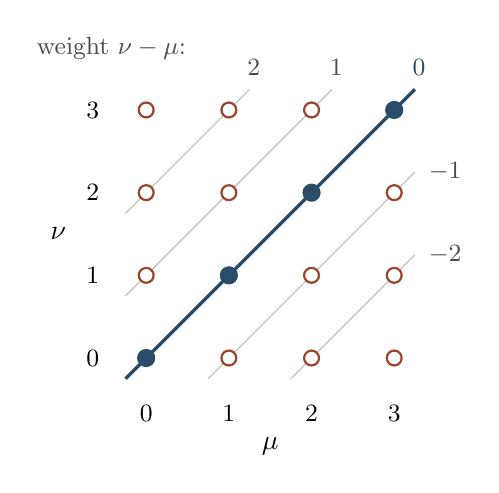
\begin{tikzpicture}[scale=1.05]
  \foreach \d in {-2,-1,1,2} {
    \pgfmathsetmacro{\xa}{max(0,-\d)} \pgfmathsetmacro{\xb}{min(3,3-\d)}
    \draw[gray!50] (\xa-0.25,\xa+\d-0.25) -- (\xb+0.25,\xb+\d+0.25);
  }
  \draw[very thick,inkblue] (-0.25,-0.25) -- (3.25,3.25);
  \foreach \m in {0,...,3} \foreach \n in {0,...,3} {
    \ifnum\m=\n \fill[inkblue] (\m,\n) circle (0.11);
    \else \draw[rust,fill=white,thick] (\m,\n) circle (0.09); \fi
  }
  \foreach \m in {0,...,3} \node[below,font=\small] at (\m,-0.45) {$\m$};
  \foreach \n in {0,...,3} \node[left,font=\small] at (-0.45,\n) {$\n$};
  \node[below] at (1.5,-0.85) {$\mu$};
  \node[left] at (-0.85,1.5) {$\nu$};
  \node[gray!60!black,font=\small,anchor=south] at (1.3,3.3) {$2$};
  \node[gray!60!black,font=\small,anchor=south] at (2.3,3.3) {$1$};
  \node[inkblue,font=\small,anchor=south] at (3.3,3.3) {$0$};
  \node[gray!60!black,font=\small,anchor=east] at (0.6,3.75) {weight $\nu-\mu$:};
  \node[gray!60!black,font=\small,anchor=west] at (3.3,2.25) {$-1$};
  \node[gray!60!black,font=\small,anchor=west] at (3.3,1.25) {$-2$};
\end{tikzpicture}
\caption{The monomials $u^\mu v^\nu$ of $G(\alpha)$ for $k=1$, placed at $(\mu,\nu)$. The weight
$\nu-\mu$ is constant along each diagonal. A homogeneous $G(\alpha)$ lives on one diagonal; the
nonzero diagonal entries $\lVert x_\mu\rVert^2$ (solid) put it on the main one, so every
off-diagonal entry $\ip{x_\mu}{x_\nu}$ (hollow) must vanish.}
\label{fig:diagonals}
\end{figure}

\begin{lemma}\label{lem:graded}
Let $R=\C[Y_1,\dots,Y_r]$ be graded by integer weights $w(Y_i)$. If $p,q\in R$ are nonzero
and $pq$ is homogeneous, then $p$ is homogeneous.
\end{lemma}

\begin{proof}
Let $a$ and $a'$ be the largest and smallest weights of monomials of $p$, and $b,b'$ those of
$q$. The weight-$(a+b)$ part of $pq$ is the product of the weight-$a$ part of $p$ and the
weight-$b$ part of $q$, since any other pair of parts has smaller total weight. Both are
nonzero and $R$ is a domain, so $pq$ has a monomial of weight $a+b$. In the same way it has
one of weight $a'+b'$. As $pq$ is homogeneous, $a+b=a'+b'$; with $a\ge a'$ and $b\ge b'$ this
forces $a=a'$.
\end{proof}

\begin{proposition}\label{prop:core}
Let $F\in P^{m\times n}$ have pairwise orthogonal coefficient matrices and vanishing $2\times2$
minors. Then $F=\alpha\beta^{\mathsf T}$ where the coefficient vectors of $\alpha$ are
pairwise orthogonal, and so are those of $\beta$.
\end{proposition}

\begin{proof}
Lemma~\ref{lem:rankone} gives $F=\alpha\beta^{\mathsf T}$. If $\alpha$ or $\beta$ is zero then
$F=0$ and there is nothing to prove, so assume both are nonzero. Some coefficient
$x_{\mu_0}$ of $\alpha$ is nonzero, and by~\eqref{eq:G} the monomial $u^{\mu_0}v^{\mu_0}$ of
$G(\alpha)$ has coefficient $\sum_i|x_{\mu_0,i}|^2>0$; in particular $G(\alpha)\ne0$, and
likewise $G(\beta)\ne0$. Fix a coordinate $j$. By~\eqref{eq:product} and
Lemma~\ref{lem:graded}, $G(\alpha)$ is homogeneous for the $j$-th weight, and the monomial
$u^{\mu_0}v^{\mu_0}$ shows that its weight is $0$. So every monomial $u^\mu v^\nu$ with
$\ip{x_\mu}{x_\nu}\ne0$ has $\nu_j=\mu_j$. This holds for every $j$, so $\ip{x_\mu}{x_\nu}\ne
0$ forces $\mu=\nu$ (Figure~\ref{fig:diagonals}). The same argument applied to $G(\beta)\,
G(\alpha)$ handles $\beta$.
\end{proof}

\section{Proof of the theorems}

\begin{proof}[Proof of Theorem~\ref{thm:sums}]
Section~\ref{sec:poly} produced $F$ with orthogonal coefficient matrices and vanishing minors.
Proposition~\ref{prop:core} gives $F=\alpha\beta^{\mathsf T}$ with orthogonal coefficient
vectors $x_\mu$ and $y_\nu$. By~\eqref{eq:torus},
\[
M(t)=e^{-ict}\alpha(z(t))\beta(z(t))^{\mathsf T}=\Bigl(\sum_\mu e^{-i(\mu\cdot\omega+c)t}
x_\mu\Bigr)\Bigl(\sum_\nu e^{-i(\nu\cdot\omega)t}y_\nu\Bigr)^{\mathsf T},
\]
which is the claim with $f_\mu=\mu\cdot\omega+c$ and $g_\nu=\nu\cdot\omega$.
\end{proof}

\begin{proof}[Proof of Theorem~\ref{thm:main}]
Apply Theorem~\ref{thm:sums} and drop the zero vectors from both families. Put
\[
h_A=\sum_\mu f_\mu\,\frac{x_\mu x_\mu^{*}}{\lVert x_\mu\rVert^2},\qquad
h_B=\sum_\nu g_\nu\,\frac{y_\nu y_\nu^{*}}{\lVert y_\nu\rVert^2}.
\]
These are Hermitian, and since the $x_\mu$ are pairwise orthogonal, $h_Ax_\mu=f_\mu x_\mu$ and
hence $e^{-ith_A}x_\mu=e^{-if_\mu t}x_\mu$; the same holds for $h_B$. With $\hat a=\sum_\mu
x_\mu$ and $\hat b=\sum_\nu y_\nu$ this gives $M(t)=e^{-ith_A}\hat a\,(e^{-ith_B}\hat b)^{
\mathsf T}$. At $t=0$ we get $\hat a\hat b^{\mathsf T}=ab^{\mathsf T}$, so $\hat a=\gamma a$
and $\hat b=\gamma^{-1}b$ for some $\gamma\ne0$, and the scalars cancel in the tensor
product.
\end{proof}

\begin{remark}
The proof is constructive once the spectrum of $H$ is known exactly. It also shows a little
more: each factor of the trajectory is an exponential sum whose frequencies lie in the group
generated by the eigenvalues of $H$, up to one common shift.
\end{remark}

\section{Constant entanglement is not enough}\label{sec:sharp}

A product state has the smallest possible entanglement. It is natural to ask whether
Theorem~\ref{thm:main} survives when ``stays a product state'' is replaced by ``keeps its
entanglement'', that is, keeps its Schmidt coefficients, so that $e^{-itH}\psi_0$ stays in the
orbit of $\psi_0$ under local unitaries. For two qubits the answer depends on the amount of
entanglement. At the other extreme from product states it is yes.

\begin{theorem}\label{thm:maxent}
Let $H$ be Hermitian on $\C^2\otimes\C^2$ and let $\psi_0$ be maximally entangled. If
$e^{-itH}\psi_0$ is maximally entangled for every $t\in\R$, then there are Hermitian $h_A$ and
$h_B$ with $e^{-itH}\psi_0=(e^{-ith_A}\otimes e^{-ith_B})\psi_0$ for all $t$.
\end{theorem}

\begin{proof}
Write the trajectory as $M(t)=\sum_{s\in S}e^{-ist}W_s$ with distinct frequencies $s$ and
nonzero, pairwise orthogonal $W_s$ (Section~2). Maximal entanglement means $M(t)M(t)^*=rI$;
taking traces, $2r=\lVert M(t)\rVert^2=\sum_s\lVert W_s\rVert^2=:q$, a constant. Hence
$\lvert\det M(t)\rvert^2=\det(MM^*)=(q/2)^2$ is constant too. Now $\det M(t)$ is a finite
exponential sum; if it had two or more frequencies with nonzero coefficients, the largest minus
the smallest would appear in $\lvert\det M(t)\rvert^2$ with a nonzero coefficient, so $\det
M(t)=\delta e^{-i\kappa t}$ for some $\delta\ne0$ and real $\kappa$.

Choose $w$ with $w^2=(q/2)/\delta$, so $\lvert w\rvert=1$, and put $N(t)=we^{i\kappa t/2}M(t)=
\sum_se^{-i(s-\kappa/2)t}W'_s$ with $W'_s=wW_s$. Then $NN^*=\tfrac q2I$ and $\det N=\tfrac q2$,
so the adjugate of $N$ equals $\det N\cdot N^{-1}=N^*$. Writing this out entrywise says
$\tau(N(t))=N(t)$ for the antiunitary involution
\[
\tau\begin{pmatrix}x_{00}&x_{01}\\ x_{10}&x_{11}\end{pmatrix}=
\begin{pmatrix}\bar x_{11}&-\bar x_{10}\\ -\bar x_{01}&\bar x_{00}\end{pmatrix},
\]
whose fixed points are the real multiples of $SU(2)$. Applying $\tau$ to the exponential sum
conjugates the phases, so comparing coefficients of distinct characters gives a pairing of the
frequencies: $\kappa-s\in S$ and $\tau(W'_{\kappa-s})=W'_s$ for every $s\in S$.

Let $T$ be the Hermitian operator on $2\times2$ matrices with eigenvectors $W'_s$ and
eigenvalues $s-\kappa/2$, and zero on their orthogonal complement. The pairing gives
$\tau T=-T\tau$. The matrices $E_0=I$, $E_1=iZ$, $E_2=iY$, $E_3=iX$ are fixed by $\tau$ and
orthogonal with $\lVert E_a\rVert^2=2$, and the two relations force
$\ip{E_a}{TE_b}=2i\,\omega_{ab}$ with $\omega$ real and antisymmetric. A direct computation
with the products of Pauli matrices shows that $TX=AX+XC$ for all $X$, where $A=\alpha\cdot
\sigma$ and $C=\gamma\cdot\sigma$ with
\[
\alpha=\tfrac12\bigl(\omega_{03}+\omega_{12},\ \omega_{02}-\omega_{13},\ \omega_{01}+\omega_{23}\bigr),
\qquad
\gamma=\tfrac12\bigl(\omega_{03}-\omega_{12},\ \omega_{02}+\omega_{13},\ \omega_{01}-\omega_{23}\bigr);
\]
this is the splitting $\mathfrak{so}(4)=\mathfrak{su}(2)\oplus\mathfrak{su}(2)$ made explicit.
Hence $A'W_s+W_sC=sW_s$ with $A'=A+\kappa/2$. In eigenbases of $A'$ and $C$ this says that
every nonzero entry of $W_s$ sits at a pair of eigenvalues $a_k+c_l=s$, so $e^{-itA'}W_s
e^{-itC}=e^{-ist}W_s$. Summing over $s$ gives $M(t)=e^{-itA'}M(0)e^{-itC}$, which is the claim
with $h_A=A'$ and $h_B=C^{\mathsf T}$.
\end{proof}

Between the two extremes the statement fails, and the counterexample is the second example of
Section~1 again.

\begin{example}
Let $H=\tfrac12(X\otimes X+Y\otimes Y+Z\otimes Z)-\tfrac12(Z\otimes1+1\otimes Z)+\tfrac32$ and
$\psi_0=-\lvert00\rangle+(1+i)\lvert01\rangle+(i-1)\lvert10\rangle+\lvert11\rangle$. The
eigenvalues of $H$ are $0,1,2,3$, on the singlet, $\lvert00\rangle$, the triplet state
$(\lvert01\rangle+\lvert10\rangle)/\sqrt2$ and $\lvert11\rangle$. With $z=e^{-it}$ the
trajectory in matrix form is
\[
M(t)=\begin{pmatrix}-z&1+iz^2\\ iz^2-1&z^3\end{pmatrix},\qquad \det M(t)=1,\qquad
\lVert M(t)\rVert^2=6 .
\]
So the squared Schmidt coefficients stay equal to $\tfrac12\pm\tfrac{\sqrt2}{3}$ for all time
and the concurrence stays $1/3$. Yet no time-independent local Hamiltonian generates this
trajectory. If $M(t)=e^{-itA}M(0)e^{-itC}$, then $\det M(t)=e^{-it(\operatorname{tr}A+
\operatorname{tr}C)}\det M(0)$, and constancy forces $\operatorname{tr}A+\operatorname{tr}C=0$.
The frequencies of such a trajectory lie among the sums $a_i+c_j$ of eigenvalues, a set that
is symmetric under negation, since $(a_1+c_1)+(a_2+c_2)=(a_1+c_2)+(a_2+c_1)=0$. The trajectory
above has frequencies $0,1,2,3$, each with a nonzero component, and no set of at most four
reals symmetric under negation contains them.
\end{example}

The mechanism is the resonance $1+3=2+2$. Expanding, $\det M(t)=(-z)(z^3)-(1+iz^2)(iz^2-1)
=-z^4-(-1-z^4)$: the term from the $\lvert00\rangle$ and $\lvert11\rangle$ components, at
frequency $1+3$, cancels the square of the triplet component, at frequency $2+2$. This is
exactly the kind of cancellation that Theorem~\ref{thm:main} had to rule out for product
states. There, rank one leaves no room for it; at intermediate entanglement there is room.

\section{Related questions}

The question~\cite{SE816017} was posed as a simplification of two harder ones. The first
replaces product states by entangled states whose entanglement does not change in time;
Section~\ref{sec:sharp} shows that the answer is then no in general, already for two qubits,
and yes for two qubits that stay maximally entangled. The second asks whether a Hamiltonian
that acts ``simply'' on every state of a subspace acts simply on the subspace as a
whole~\cite{SE797030}, and remains open as far as we know. A related question about
non-entangling bases of bipartite unitaries is~\cite{SE602903}.

\section{Formal verification}

The Lean~4 development~\cite{mathlib} proves Theorem~\ref{thm:sums} in the form stated above,
from the hypotheses~\eqref{eq:M} (an arbitrary finite family of reals $\lambda_j$, repeats
allowed, and pairwise orthogonal matrices $V_j$) and the hypothesis that $M(t)$ is a column
times a row for every real $t$. It contains Lemmas~\ref{lem:lattice} to~\ref{lem:graded} and
Proposition~\ref{prop:core}, with Dedekind's lemma, unique factorisation of polynomial rings
and the existence of bases of finitely generated free abelian groups taken from Mathlib. The
main theorem depends only on the standard axioms (propositional extensionality, choice and
quotient soundness). Mutants, each weakening one hypothesis or strengthening one conclusion, fail
to check (counted below). The two steps outside the formal development are standard
linear algebra: the spectral decomposition at the start of Section~2, and the construction of
$h_A$ and $h_B$ from orthogonal vectors in the proof of Theorem~\ref{thm:main}, together with
the induction of Corollary~\ref{cor:multi}. A short computation in exact rational arithmetic,
independent of the Lean code, runs the construction on degenerate and resonant
examples with one and two independent frequencies.

Section~\ref{sec:sharp} is formalised as well. Theorem~\ref{thm:maxent} is proved in the
exponential-sum form used in its proof, with the same route: the single-frequency lemma for
constant-modulus sums, the involution $\tau$, the pairing by comparison of coefficients, the
explicit splitting of $\mathfrak{so}(4)$, and the evolution of eigenvectors of $X\mapsto AX+XC$.
For the Example, Lean checks the eigen-equations of $H$ in Pauli form, the expansion of
$M(t)$ into orthogonal components, $\det M(t)=1$ and $\lVert M(t)\rVert^2=6$, and that no
Hermitian $A$ and $C$ satisfy $M(t)=e^{-itA}M(0)e^{-itC}$ for all $t$, using the matrix
exponential of Mathlib. All of these depend only on the standard axioms, and twenty-six mutants
in total fail to check. The Lean files and both exact computations are at~\cite{repo}.

\paragraph{Acknowledgments.} The question was posed on Physics Stack Exchange by
\texttt{user196574}, and Norbert Schuch's comment there reduced it to the bipartite case.
Anthropic's Claude (Opus~5.5) was used to search the literature, develop and check the proof,
write the Lean formalisation and the exact computation, and draft this text. The author
is responsible for the content of this preprint, which has not yet been independently reviewed.

\begin{thebibliography}{9}
\bibitem{repo}
V. Jandhyala, When a product state stays a product state: Lean proofs and code,
\url{https://github.com/jvvk/mathematics/tree/main/product-state-trajectories}.

\bibitem{Durt2001}
T. Durt, Characterisation of an entanglement-free evolution, preprint (2001),
arXiv:quant-ph/0109112.

\bibitem{Durt2004}
T. Durt, Quantum entanglement, interaction, and the classical limit, \emph{Z. Naturforsch. A}
\textbf{59} (2004), 425--436, doi:10.1515/zna-2004-7-805.

\bibitem{Lang}
S. Lang, \emph{Algebra}, revised third edition, Graduate Texts in Mathematics 211, Springer,
New York, 2002, doi:10.1007/978-1-4613-0041-0.

\bibitem{mathlib}
The mathlib Community, The Lean mathematical library, in \emph{Proceedings of the 9th ACM
SIGPLAN International Conference on Certified Programs and Proofs (CPP 2020)}, ACM, New
York, 2020, 367--381.

\bibitem{SE602903}
user6873235, Do bipartite unitary operators always have a ``non-entangling'' basis?, Physics
Stack Exchange, question 602903, 25 December 2020,
\url{https://physics.stackexchange.com/q/602903} (accessed 14 October 2026).

\bibitem{SE797030}
user196574, A Hamiltonian acts simply on each state in some subspace. Can it be identified with
a single simple operator on the subspace?, Physics Stack Exchange, question 797030, 12 January
2024, \url{https://physics.stackexchange.com/q/797030} (accessed 14 October 2026).

\bibitem{SE816017}
user196574, Time evolution keeps a certain product state always a product state. Is there a
time-independent factorizable evolution for this state?, Physics Stack Exchange, question
816017, 26 May 2024, \url{https://physics.stackexchange.com/q/816017} (accessed 14 October
2026).

\bibitem{SperlingWalmsley}
J. Sperling and I. A. Walmsley, Separable and inseparable quantum trajectories, \emph{Phys.
Rev. Lett.} \textbf{119} (2017), 170401, doi:10.1103/PhysRevLett.119.170401.
\end{thebibliography}

\end{document}
